\section{Results}
\label{results_convergence_checking}


\subsection{Convergence monitoring}
\label{subsection_convergence}

Before making inferences using posterior simulations generated by an MCMC algorithm 
it is essential to check for evidence of convergence to the target distribution. Although this 
process is not an exact science, there is no shortage of literature on the topic of monitoring 
convergence for MCMC and other iterative simulation algorithms. The various convergence 
diagnostics used below are introduced informally. Formal definitions, computational details, 
and recommended best practices can be found in \citeA{gelman_handbook_2011}, 
\citeA{gelman_bayesian_2013}, and \citeA{stan_development_team_stan_2015}.

Eight randomly initialized chains of 2000 iterations (including a warmup period of 1000 
discarded draws) were simulated.\footnote{Newcomers to HMC, NUTS, and Stan are 
often surprised by how few iterations are typically required, as it is not uncommon for 
Gibbs (and poorly tuned M-H) samplers to require hundreds of thousands of iterations 
to converge. Simpler models fit in Stan often require only hundreds of iterations, including 
warmup. This is due in large part to the advantages of HMC discussed in \ref{stan_intro}, in
particular the suppression of random walk behavior leading to more efficient exploration
of the parameter space.} 

In Figure~\ref{fig:ck_diagnostics}, panel ({\bf a}) shows the distribution of the estimates of 
the potential scale reduction statistic $\hat{R}$  \shortcite{gelman_rhat_1992}. The $\hat{R}$ 
statistic is a comparison of the variance of the simulations within individual chains to that of 
the simulations when chains are pooled. Here, the distribution of $\hat{R}$ shows that for 
all parameters the value is approximately one, indicating that little would be gained by running 
longer chains \shortcite{gelman_handbook_2011}. 

\begin{figure}
\centering
	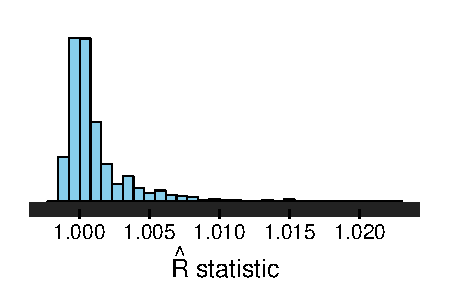
\includegraphics[scale=0.7]{sections/figs/rhat}
	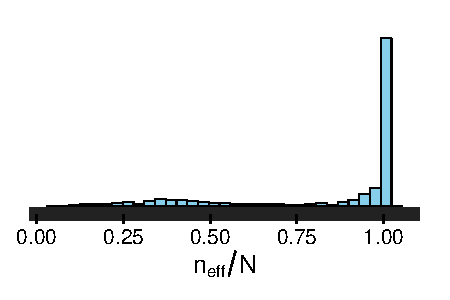
\includegraphics[scale=0.7]{sections/figs/neff}
	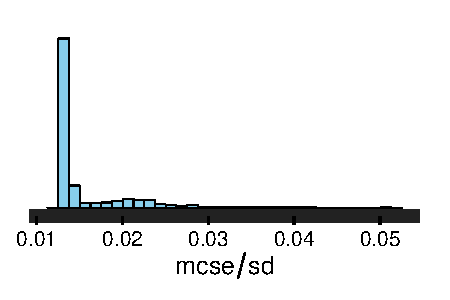
\includegraphics[scale=0.7]{sections/figs/mcse}
\caption{Distributions of diagnostics computed from the MCMC draws. 
From left to right: \newline ({\bf a}) Potential scale reduction factor $\hat{R}$ \newline ({\bf b}) 
Ratio of effective sample size to total sample size ($n_{\it eff}/N$) \newline ({\bf c}) Ratio of 
Monte Carlo error to posterior standard deviation ($mcse/sd$)}
\label{fig:ck_diagnostics}
\end{figure}

Panel ({\bf b}) shows the distribution of the ratio of effective sample size to the number of 
iterations ($n_{\it eff}/N$). Roughly speaking, $n_{\it eff}$ is an estimate of the number of 
{\it independent} draws from the posterior distribution that would have the same expected 
variance as the $N$ {\it dependent} draws actually obtained from the 
Markov chains. In the absence of autocorrelation $n_{\it eff} = N$, and so the ideal value of the ratio is one. 
In this case $n_{\it eff}/N$ is sufficiently large -- it is at least 20\% for all parameters -- and 
for most parameters the ratio is close to one, a reflection of Stan's efficiency. 


The distribution of the ratio of Monte Carlo error to the estimated standard 
deviation ($mcse/sd$) is shown in panel ({\bf c}) of Figure~\ref{fig:ck_diagnostics}. 
Monte Carlo error is a measure of imprecision due to approximating 
the posterior distribution by the MCMC simulations. As the number of iterations increases 
$mcse$ tends toward zero and the standard deviation of the draws converges to the posterior 
standard deviation. In this case, for all parameters the relative error $mcse/sd$ is less 
than five percent, which, for the inferential goals of this analysis, is negligible. 

For example, Figure~\ref{fig:ck_example_posterior} shows the estimated 
posterior density for the parameter corresponding to bias towards the majority party in the 79th 
congress.\footnote{There is nothing special about the 79th congress for this purpose. A single 
congress was chosen at random to use as an example.} The posterior is approximately Gaussian, 
with mean and standard deviation of roughly $0.054$ and $0.037$, respectively. The 
estimated $mcse$ is $0.0007$, which is inconsequential when compared to the uncertainty about 
the parameter in the posterior distribution.   


\begin{figure}[h]
\centering
	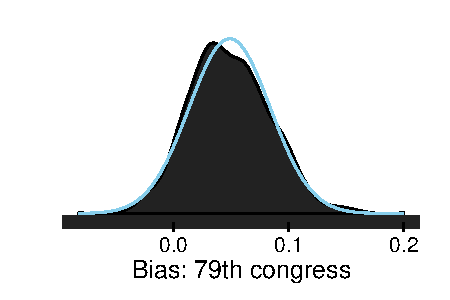
\includegraphics[scale=0.75]{sections/figs/example_posterior}
\caption{Posterior kernel density estimate for bias towards the majority party in the 79th congress. 
Normal density curve in blue.}
\label{fig:ck_example_posterior}
\end{figure}


%DEPENDENCE PLOT?
%
%
%\begin{figure}[h]
%\centering
%	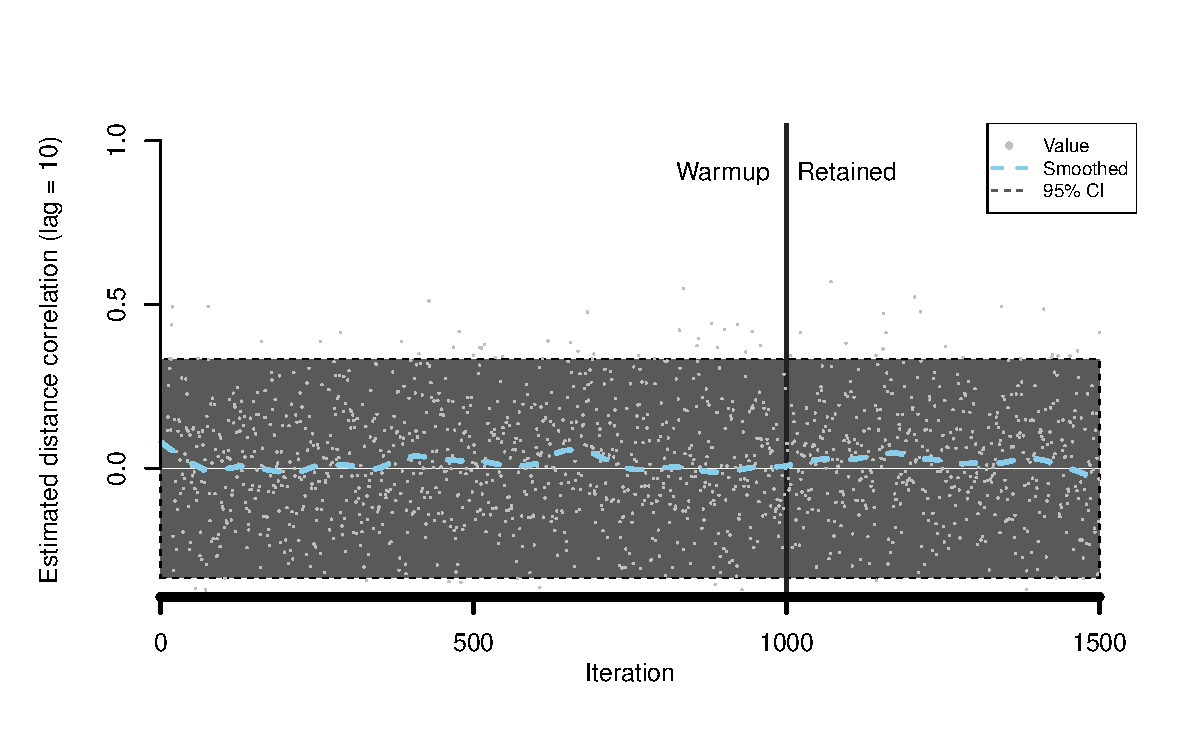
\includegraphics[scale=0.75]{sections/figs/ck_dependence}
%\caption{Estimated distance correlation among the eight chains. At a lag of 10 the draws are essentially independent. }
%\label{fig:ck_dependence}
%\end{figure}
%

In addition to the diagnostics discussed above, trace plots for all parameters were also 
examined as well as additional quantities specific to HMC and NUTS.\footnote{For example, 
checking that the tree depth used by NUTS is well below the user-specified maximum, ensuring 
that there are no post-warmup leapfrog iterations with diverging error, etc. These are explained 
in greater detail in \citeA{stan_development_team_stan_2015}.}

See Appendix F (p.~\pageref{AppendixF}) % Appendix~\ref{AppendixF} 
for graphical posterior predictive model checking. 


\subsection[Estimates and discussion]{Estimated bias toward the majority party}
\label{results}

\subsubsection{Comparing the results}

Figure~\ref{fig:ck_bias} (p.~\pageref{fig:ck_bias}) juxtaposes the estimates of 
bias towards the majority party over time from Cox and Katz's analysis and the reanalysis 
using the Bayesian STAR model.

\begin{figure}
\centering
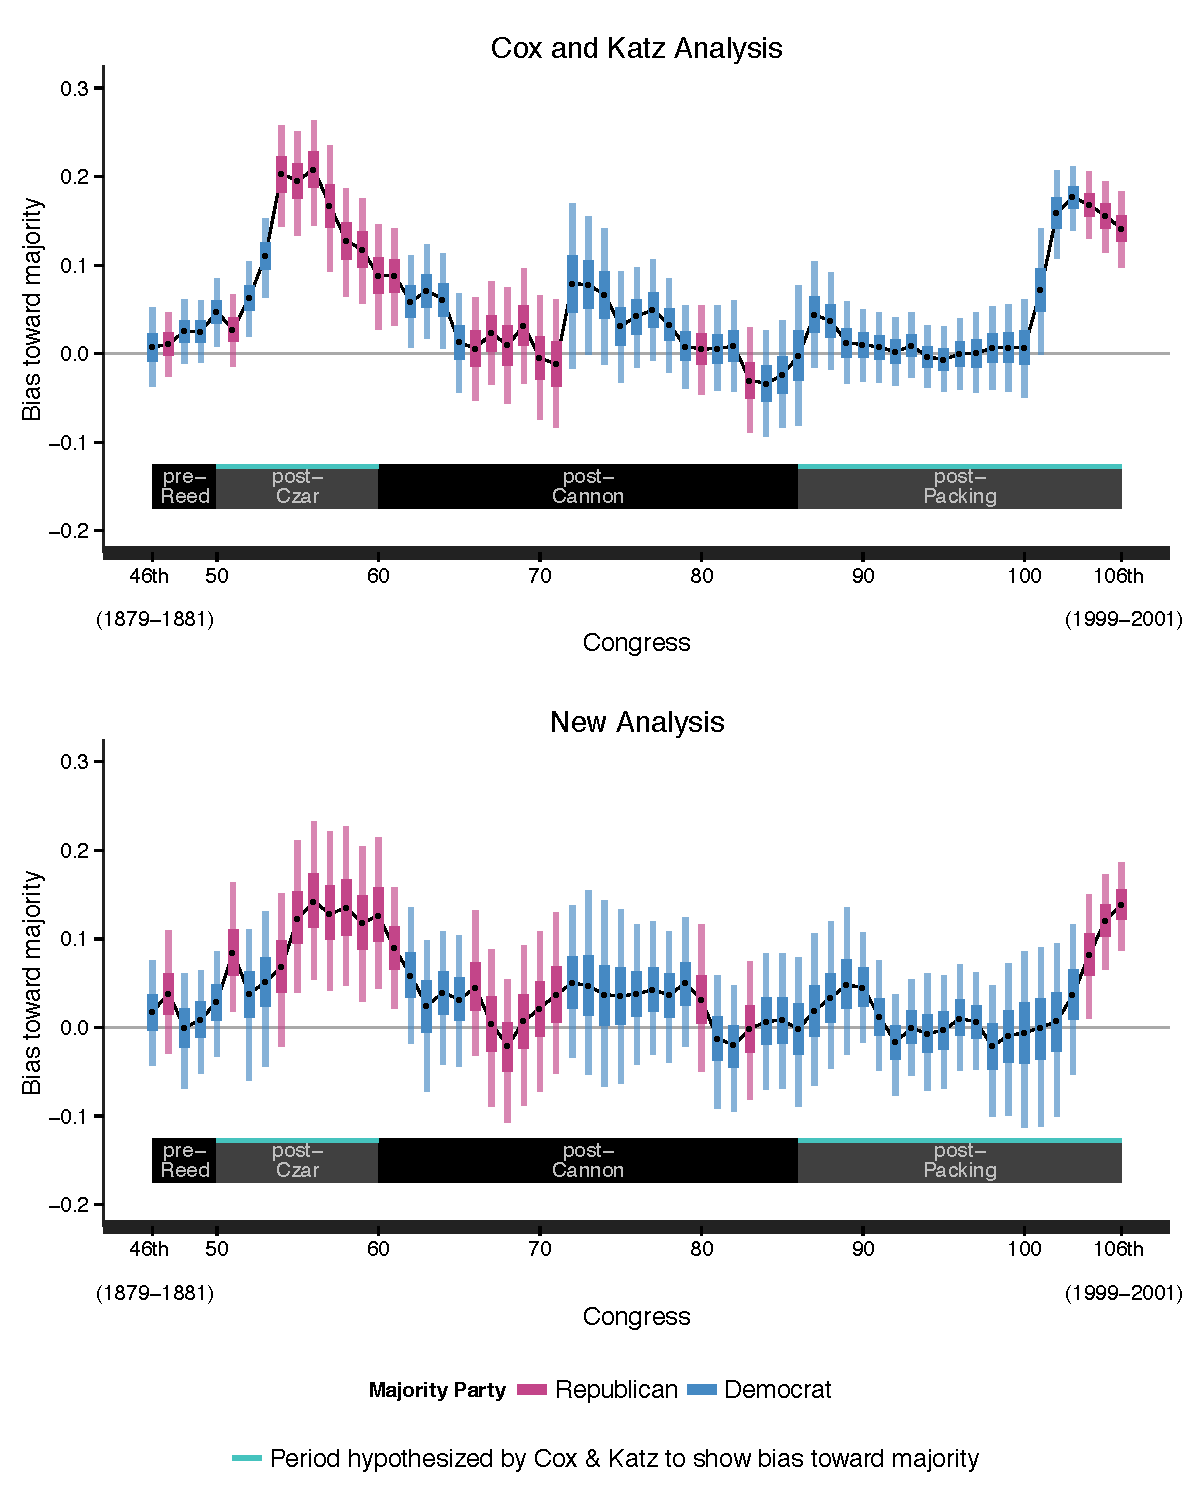
\includegraphics[scale=0.75]{sections/figs/ck_replication_new}
\caption{Estimated bias toward the majority party by Congress in 
Cox and Katz's analysis (top) and the Bayesian reanalysis (bottom). 
The thin and thick vertical segments represent 95\%  and 50\%
intervals, respectively.  The black line connects medians.
To produce the graph on top Cox and Katz's original analysis was 
replicated (see Figure 3 in Cox and Katz (2007)).}
\label{fig:ck_bias}
\end{figure}

Immediately noticeable is that the new estimates have greater 
uncertainties, which is to be expected due to the potential for Cox and Katz's method to 
produce overly precise estimates  (see section \ref{subsection_methods}). The new results 
do provide some support for the hypothesis of bias during the post-czar and post-packing 
periods; the evidence is much weaker than that found by Cox and Katz, but the finding 
of bias toward the Republican majority in the latter half of the post-czar period holds up. 

When compared to Cox and Katz's results, the hierarchical Bayesian STAR model estimates 
a more believable trend in bias over time. This can be seen clearly by comparing the curves 
in Figure~\ref{fig:ck_bias}. The smoothing prior shrinks each individual estimate slightly 
towards its neighbors -- the amount of smoothing is related to the hierarchical variance 
hyperparameter -- and all estimates are shrunk to the common prior mean, which helps 
avoid overfitting but still allows for substantial movement between Congresses 
if strongly supported by the data. Although both sets of results agree on the direction of 
bias in the post-czar period, while the Cox and Katz estimates show signs of overfitting 
the new estimates are less volatile. 


\subsubsection{Problems with statistical significance}

Cox and Katz proceed with inference by comparing the statistical significance of their 
estimates. This is problematic for for several reasons.\footnote{``In the czar-rule era, 
the running average bias is statistically significant in nine out of ten Congresses \dots", } 
First, if the reported standard errors understate the uncertainty in their estimates 
-- and this is presumably the case, as emphasized above and in \ref{subsection_methods} 
-- then they will be more likely to find statistical significance than is justified from the data, 
regardless of the arbitrary threshold selected for determining significance. Second, there
are numerous cases in which the difference between statistically significant 
bias in Congress $t$ and nonsignificant bias in Congress $t + 1$ (or vice-versa) is not itself 
statistically significant. 

Three such examples are given in Figure~\ref{fig:ck_signif}. The plot on the left, for instance, 
shows Cox and Katz's point estimates and 95\% intervals for bias in the 100th and 101st 
Congresses. The estimates (plus or minus one standard error) are $b_{100} = 0.0065 \pm 0.029$ 
and $b_{101} = 0.071 \pm 0.034$. Assuming the 95\% threshold for statistical significance 
standard in the social sciences and used by Cox and Katz, $b_{101}$ is statistically significant 
but $b_{100}$ is not. Though it is then tempting to conclude that one is signal while the other 
is indistinguishable from noise, note that the difference between the two is 
$0.0645$ with a standard error of $0.045$ and thus not close to statistically significant. 
The general point is counter-intuitive: nonsignificant changes can correspond to large shifts 
in significance levels.\footnote{A more detailed explanation of this issue -- which is not unique to this 
example -- and its potential consequences can be found in Chapter 2 of 
\citeA{gelman_arm_2007}.}\footnote{The same concern would arise to some extent if the filter 
of statistical significance were imposed on the Bayesian analysis, but it is not the natural framework 
for making inferences from a Bayesian perspective.} 

For a discussion of the interpretation of confidence intervals in the context of Cox and Katz's analysis 
see Appendix E (p.~\pageref{AppendixE}). % Appendix~\ref{AppendixE}. 

\begin{figure}
\centering
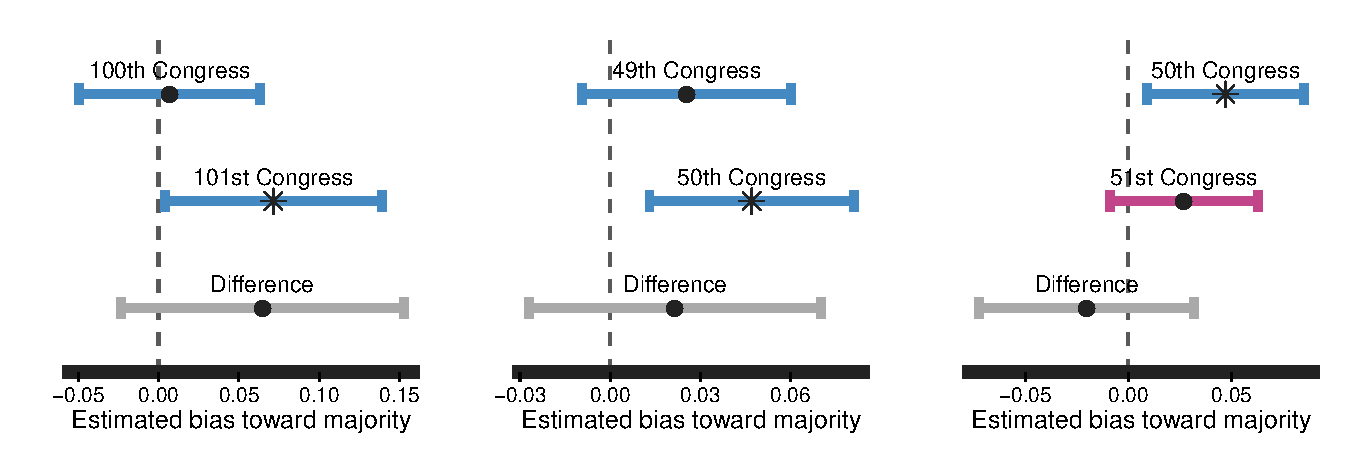
\includegraphics[scale=0.75]{sections/figs/ck_signif_all}%
%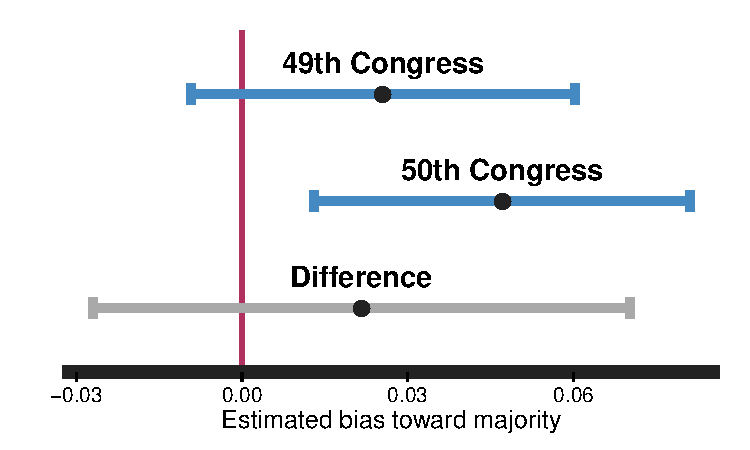
\includegraphics[scale=0.5]{sections/figs/ck_signif2}
\caption{Examples from Cox and Katz's results for which the difference between statistically 
significant and nonsignificant is not itself statistically significant.}
\label{fig:ck_signif}
\end{figure}

\subsubsection{Implications of Cox and Katz's rolling average approach}

As discussed in \ref{subsection_methods}, Cox and Katz's results comprise estimates taken 
from 61 separate models (one for each Congress). This results in the data for each Congress 
$t$ being reused in up to six of the 60 models besides the model for Congress $t$ itself. It also 
entails the exclusion of all data from Congresses outside each window. Furthermore, the 
choice of using rolling windows of seven Congresses ($t \pm 3$) is somewhat arbitrary. 

\begin{figure}
\centering
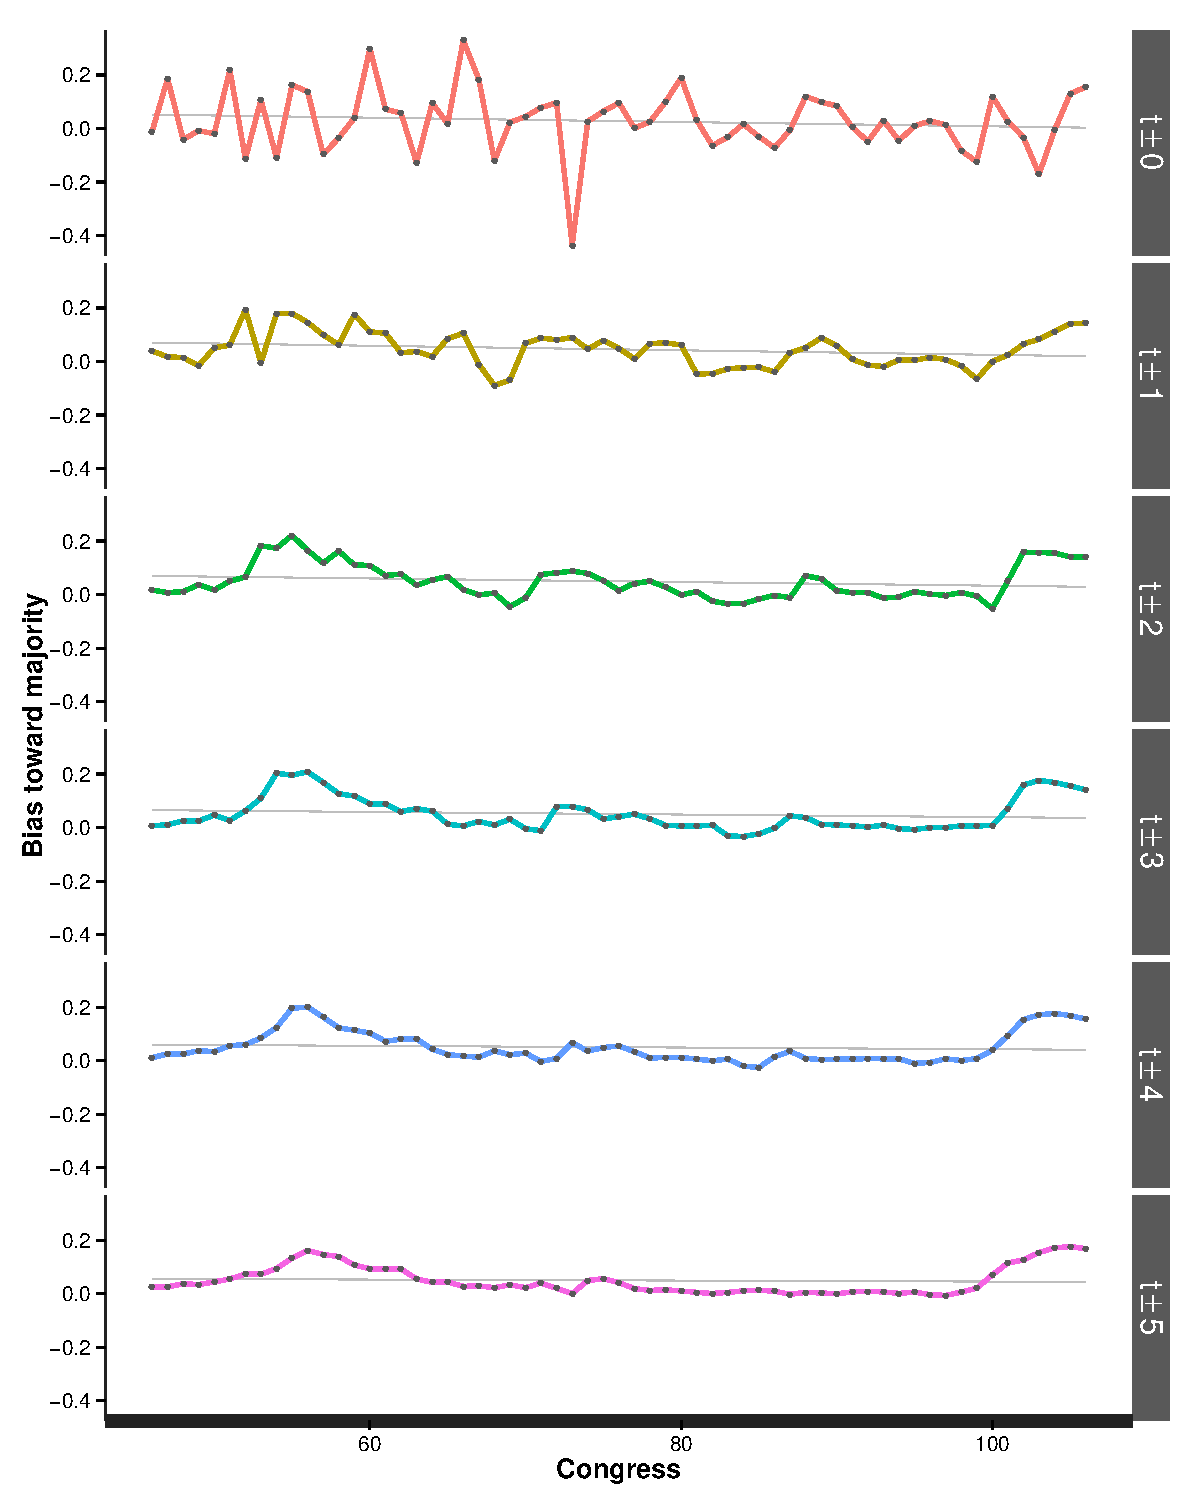
\includegraphics[scale=0.75]{sections/figs/ck_hypothetical}
\caption{Replications of Cox and Katz's results but changing the number of Congresses 
included when estimating each point. The top panel corresponds to estimating bias in each 
Congress $t$ using only data from time $t$ (i.e., $t \pm 0$). In each subsequent panel the 
set of Congresses is expanded by one in both directions. The bottom panel corresponds to 
using $t \pm 5$. The analysis presented in \protect\citeA{cox_gerrymandering_2007} is the 
panel for $t \pm 3$. The horizontal gray lines are the estimates obtained by completely 
pooling the data from all Congresses. Error bars are excluded so that differences in the 
smoothness of the curves are more perceptible.}
\label{fig:ck_hypothetical}
\end{figure}


The curves in Figure~\ref{fig:ck_hypothetical} (p.~\pageref{fig:ck_hypothetical}) show the 
results Cox and Katz would have found had they chosen narrower or wider windows. As the 
set of Congresses included in each model grows, the resulting curve necessarily becomes 
smoother because Cox and Katz's method is less and less distinguishable from simply 
estimating a common bias parameter for all Congresses (that is, assuming no variation in 
bias over time). Conversely, the single Bayesian model -- via the smoothness prior and the 
model's hierarchical structure -- allows for bias in each Congress to depend on neighboring 
Congresses while using the entire dataset only once, obviating the need to dubiously subset 
the data. 



